\documentclass[11pt]{article}
\usepackage[textwidth=18.0cm, textheight=23.0cm, top=2.0cm]{geometry}
\usepackage{pst-all}
\usepackage{amssymb}
\usepackage{tikz}
\usepackage{underscore}\begin{document}
\pagestyle{empty}


ClassName: \underline{\textbf{Class_10.2bp-17}}
\par
BinSize: \underline{\textbf{100 × 100}}
\par
ReduceSize: \underline{\textbf{100 × 100}}
\par
TypeNum: \underline{\textbf{39}}
\par
Num: \underline{\textbf{40}}
\par
OutS: \underline{\textbf{70000}}
\par
InS: \underline{\textbf{61000}}
\par
Rate: \underline{\textbf{0.871}}
\par
UB: \underline{\textbf{7}}
\par
LB0: \underline{\textbf{7}}
\par
LB: \underline{\textbf{7}}
\par
LBWithCut: \underline{\textbf{7}}
\par
NodeCut: \underline{\textbf{0}}
\par
ExtendedNodeCnt: \underline{\textbf{1}}
\par
GenNodeCnt: \underline{\textbf{1}}
\par
PrimalNode: \underline{\textbf{0}}
\par
ColumnCount: \underline{\textbf{7}}
\par
TotalCutCount: \underline{\textbf{0}}
\par
RootCutCount: \underline{\textbf{0}}
\par
LPSolverCnt: \underline{\textbf{1}}
\par
PricingSolverCnt: \underline{\textbf{0}}
\par
BranchAndBoundNum: \underline{\textbf{1}}
\par
isOpt: \underline{\textbf{true}}
\par
TimeOnInitSolution: \underline{\textbf{0.030 s}}
\par
TimeOnPrimal: \underline{\textbf{0.000 s}}
\par
TimeOnPricing: \underline{\textbf{0.000 s}}
\par
TimeOnRmp: \underline{\textbf{0.078 s}}
\par
TotalTime: \underline{\textbf{0.155 s}}
\par
\newpage


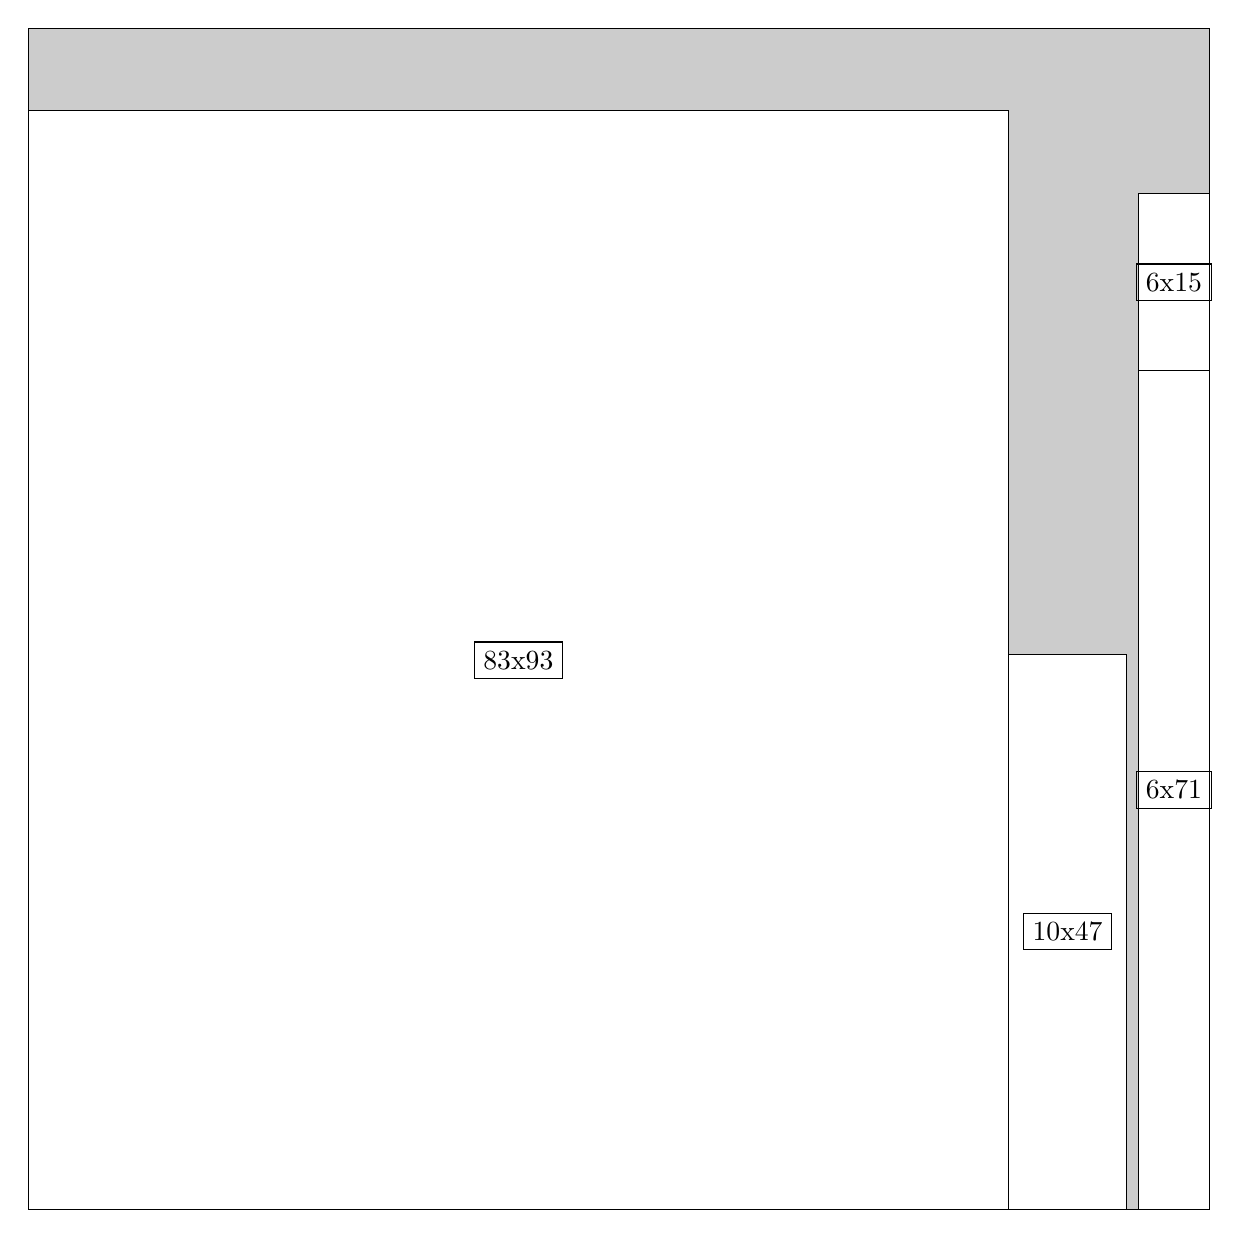
\begin{tikzpicture}[shorten >=1pt,scale=1.0,every node/.style={scale=1.0},->]
\tikzstyle{vertex}=[circle,fill=black!25,minimum size=14pt,inner sep=0pt]
\filldraw[fill=gray!40!white, draw=black] (0,0) rectangle (15.0,15.0);
\foreach \name/\x/\y/\w/\h in {83x93/0.0/0.0/12.45/13.95,10x47/12.45/0.0/1.5/7.05,6x71/14.1/0.0/0.8999999999999999/10.65,6x15/14.1/10.65/0.8999999999999999/2.25}
\filldraw[fill=white!40!white, draw=black] (\x,\y) rectangle node[draw] (\name) {\name} ++(\w,\h);
\end{tikzpicture}


w =83 , h =93 , x =0 , y =0 , v =7719
\par
w =10 , h =47 , x =83 , y =0 , v =470
\par
w =6 , h =71 , x =94 , y =0 , v =426
\par
w =6 , h =15 , x =94 , y =71 , v =90
\par
\newpage


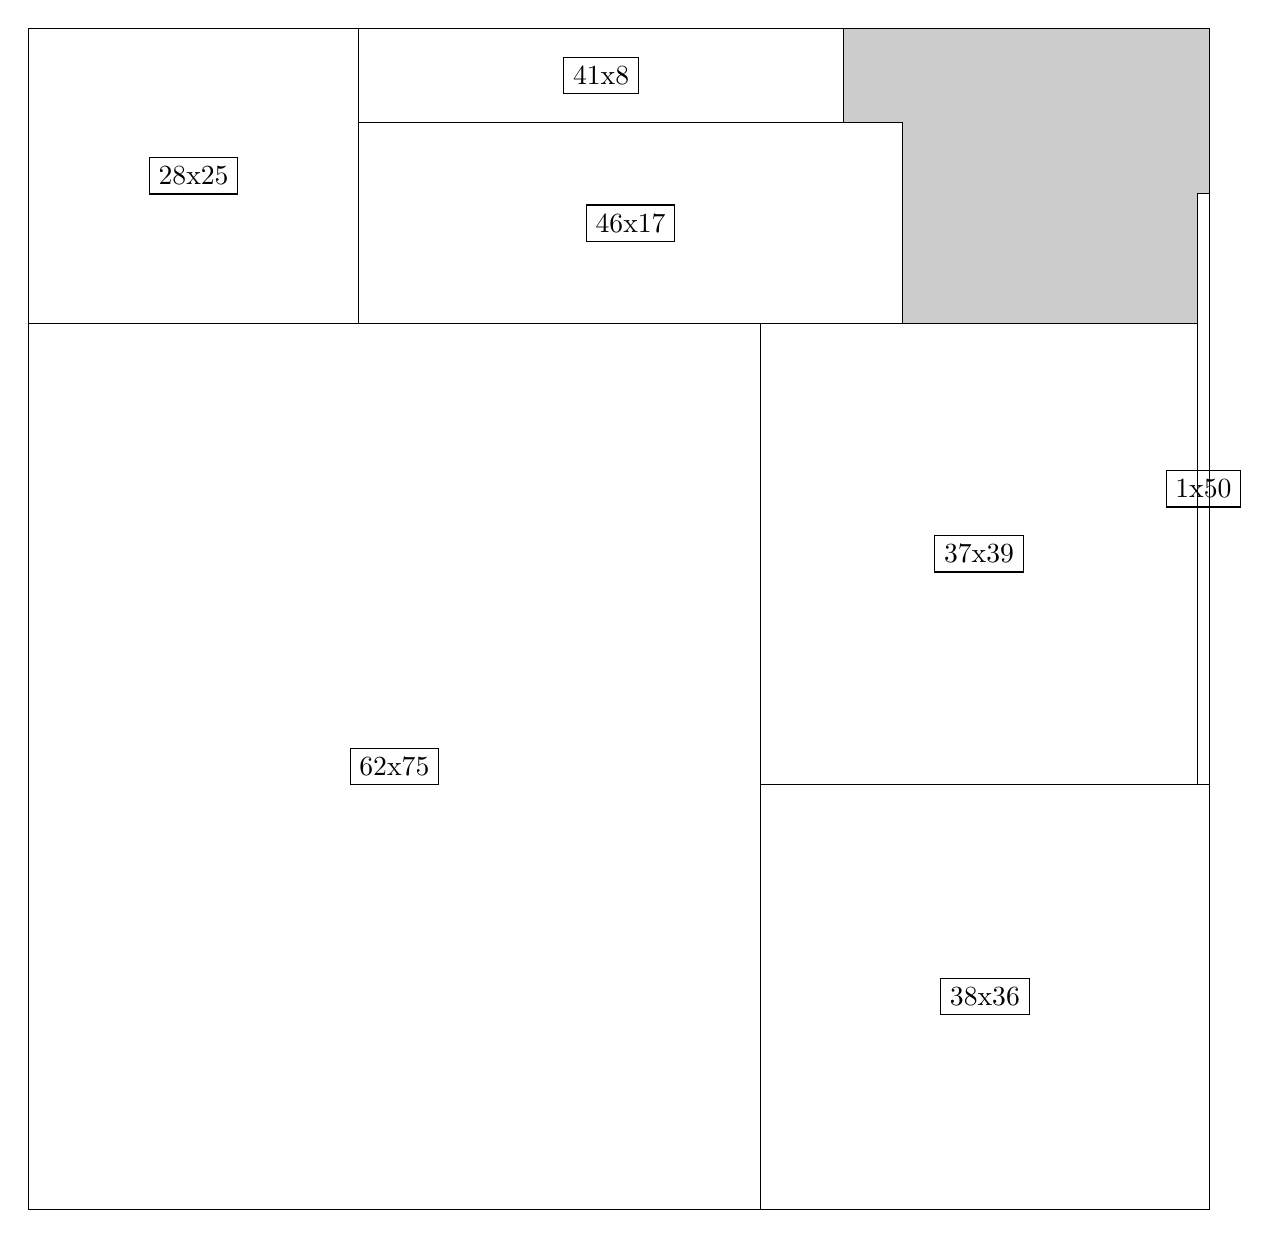
\begin{tikzpicture}[shorten >=1pt,scale=1.0,every node/.style={scale=1.0},->]
\tikzstyle{vertex}=[circle,fill=black!25,minimum size=14pt,inner sep=0pt]
\filldraw[fill=gray!40!white, draw=black] (0,0) rectangle (15.0,15.0);
\foreach \name/\x/\y/\w/\h in {62x75/0.0/0.0/9.299999999999999/11.25,37x39/9.299999999999999/5.3999999999999995/5.55/5.85,38x36/9.299999999999999/0.0/5.7/5.3999999999999995,46x17/4.2/11.25/6.8999999999999995/2.55,28x25/0.0/11.25/4.2/3.75,41x8/4.2/13.799999999999999/6.1499999999999995/1.2,1x50/14.85/5.3999999999999995/0.15/7.5}
\filldraw[fill=white!40!white, draw=black] (\x,\y) rectangle node[draw] (\name) {\name} ++(\w,\h);
\end{tikzpicture}


w =62 , h =75 , x =0 , y =0 , v =4650
\par
w =37 , h =39 , x =62 , y =36 , v =1443
\par
w =38 , h =36 , x =62 , y =0 , v =1368
\par
w =46 , h =17 , x =28 , y =75 , v =782
\par
w =28 , h =25 , x =0 , y =75 , v =700
\par
w =41 , h =8 , x =28 , y =92 , v =328
\par
w =1 , h =50 , x =99 , y =36 , v =50
\par
\newpage


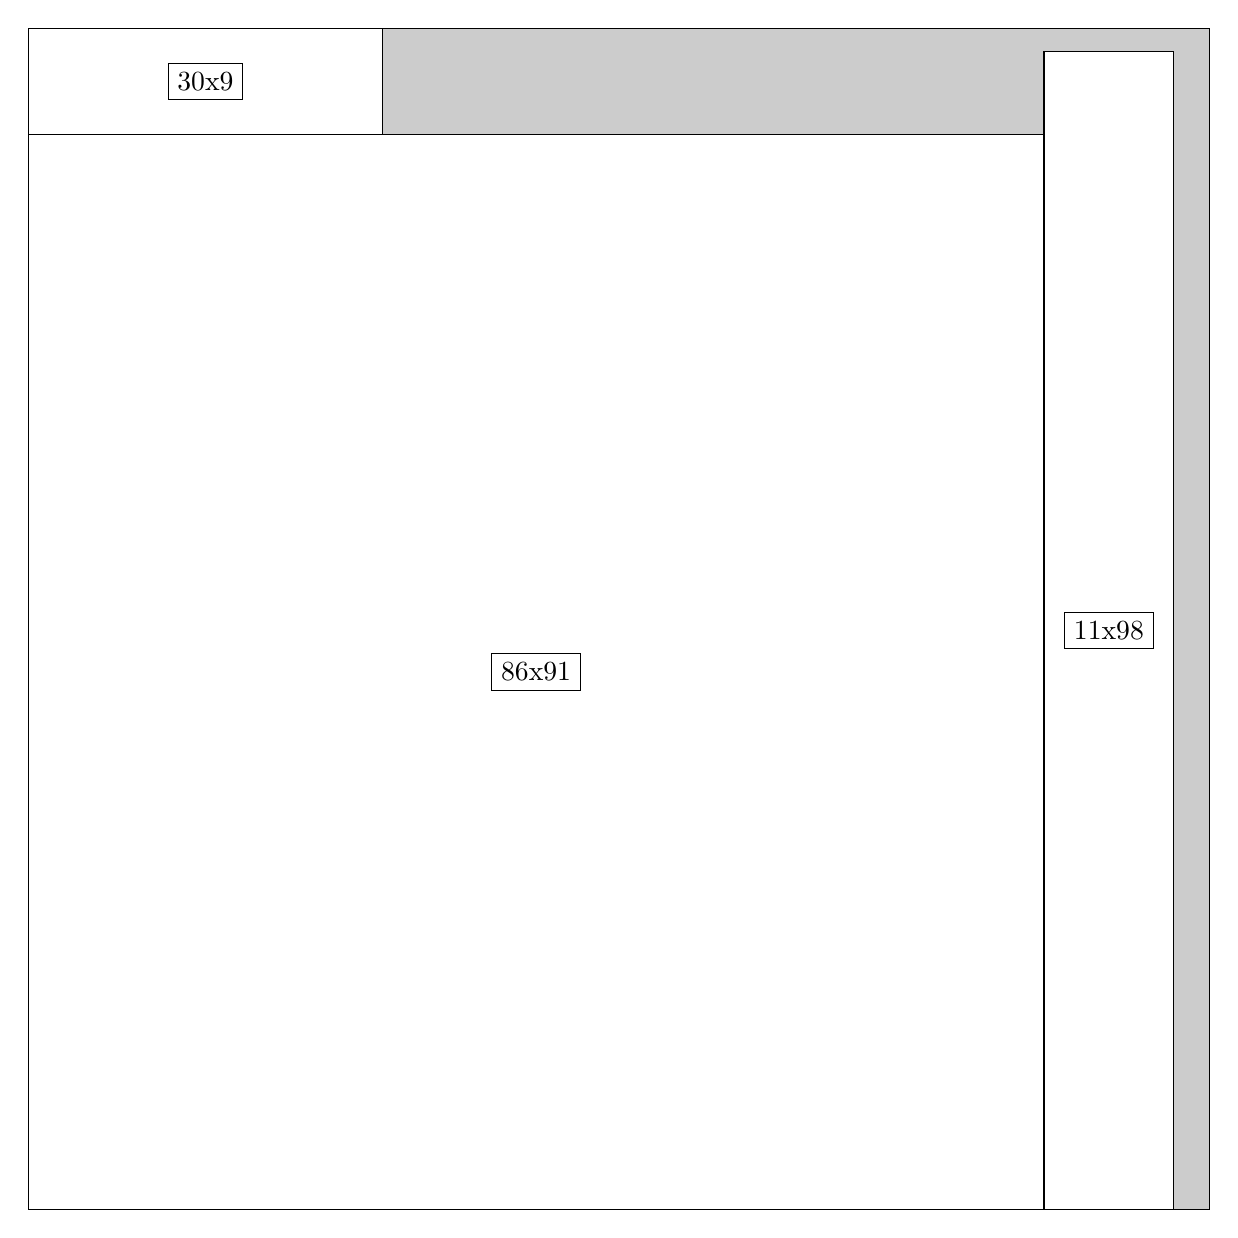
\begin{tikzpicture}[shorten >=1pt,scale=1.0,every node/.style={scale=1.0},->]
\tikzstyle{vertex}=[circle,fill=black!25,minimum size=14pt,inner sep=0pt]
\filldraw[fill=gray!40!white, draw=black] (0,0) rectangle (15.0,15.0);
\foreach \name/\x/\y/\w/\h in {86x91/0.0/0.0/12.9/13.65,11x98/12.9/0.0/1.65/14.7,30x9/0.0/13.65/4.5/1.3499999999999999}
\filldraw[fill=white!40!white, draw=black] (\x,\y) rectangle node[draw] (\name) {\name} ++(\w,\h);
\end{tikzpicture}


w =86 , h =91 , x =0 , y =0 , v =7826
\par
w =11 , h =98 , x =86 , y =0 , v =1078
\par
w =30 , h =9 , x =0 , y =91 , v =270
\par
\newpage


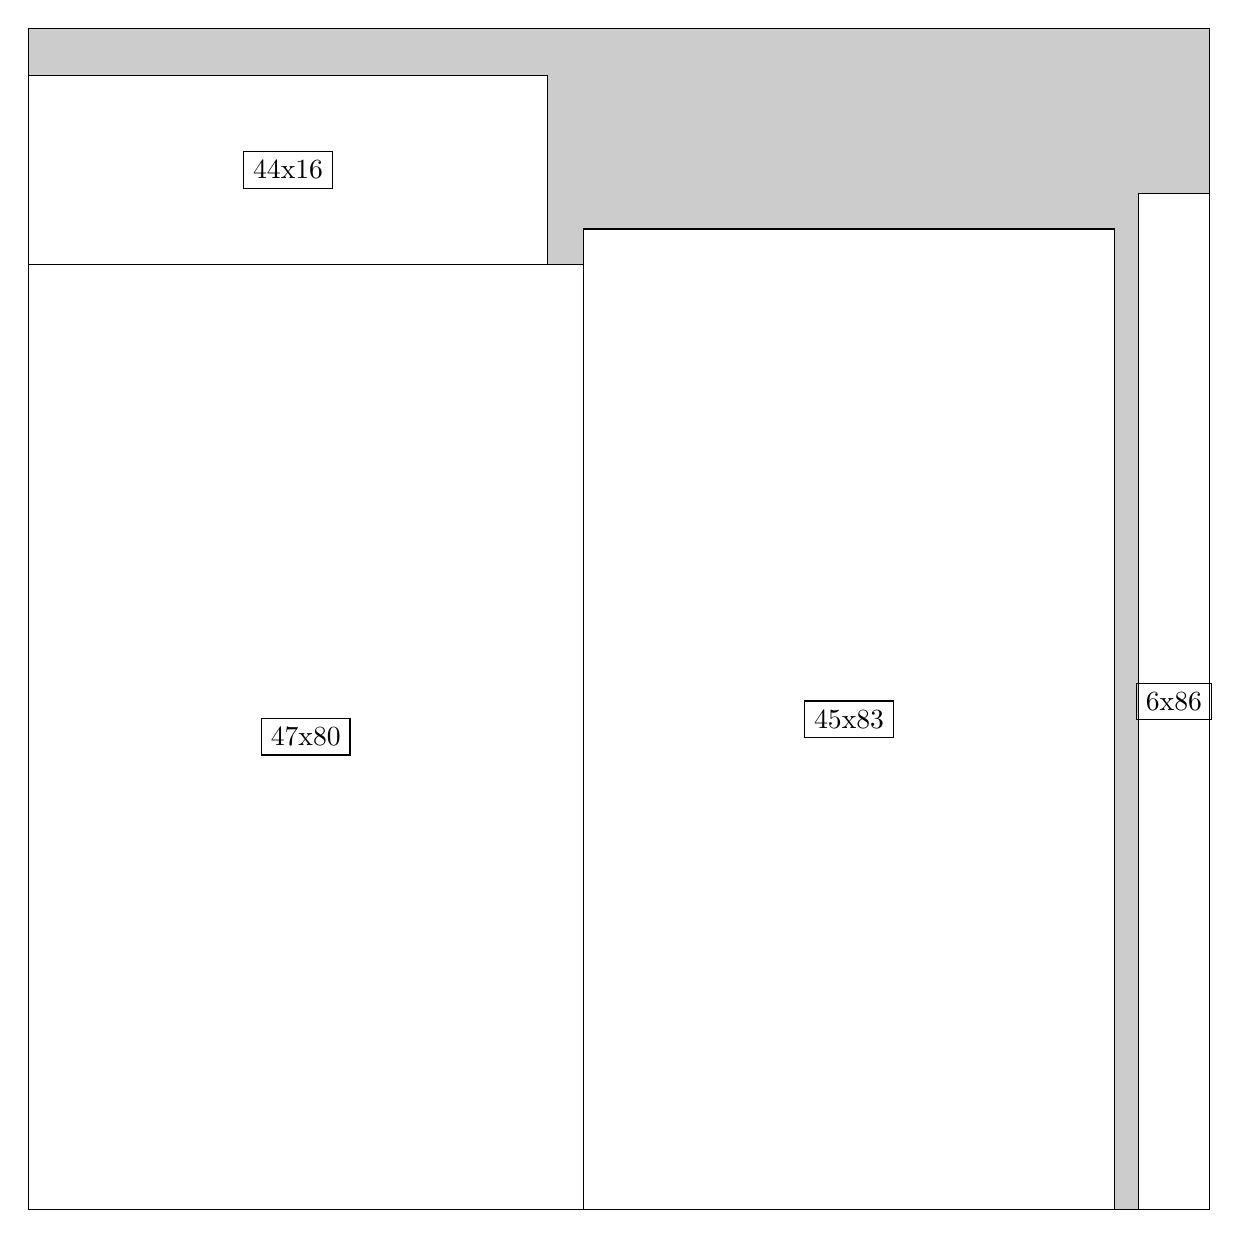
\begin{tikzpicture}[shorten >=1pt,scale=1.0,every node/.style={scale=1.0},->]
\tikzstyle{vertex}=[circle,fill=black!25,minimum size=14pt,inner sep=0pt]
\filldraw[fill=gray!40!white, draw=black] (0,0) rectangle (15.0,15.0);
\foreach \name/\x/\y/\w/\h in {47x80/0.0/0.0/7.05/12.0,45x83/7.05/0.0/6.75/12.45,44x16/0.0/12.0/6.6/2.4,6x86/14.1/0.0/0.8999999999999999/12.9}
\filldraw[fill=white!40!white, draw=black] (\x,\y) rectangle node[draw] (\name) {\name} ++(\w,\h);
\end{tikzpicture}


w =47 , h =80 , x =0 , y =0 , v =3760
\par
w =45 , h =83 , x =47 , y =0 , v =3735
\par
w =44 , h =16 , x =0 , y =80 , v =704
\par
w =6 , h =86 , x =94 , y =0 , v =516
\par
\newpage


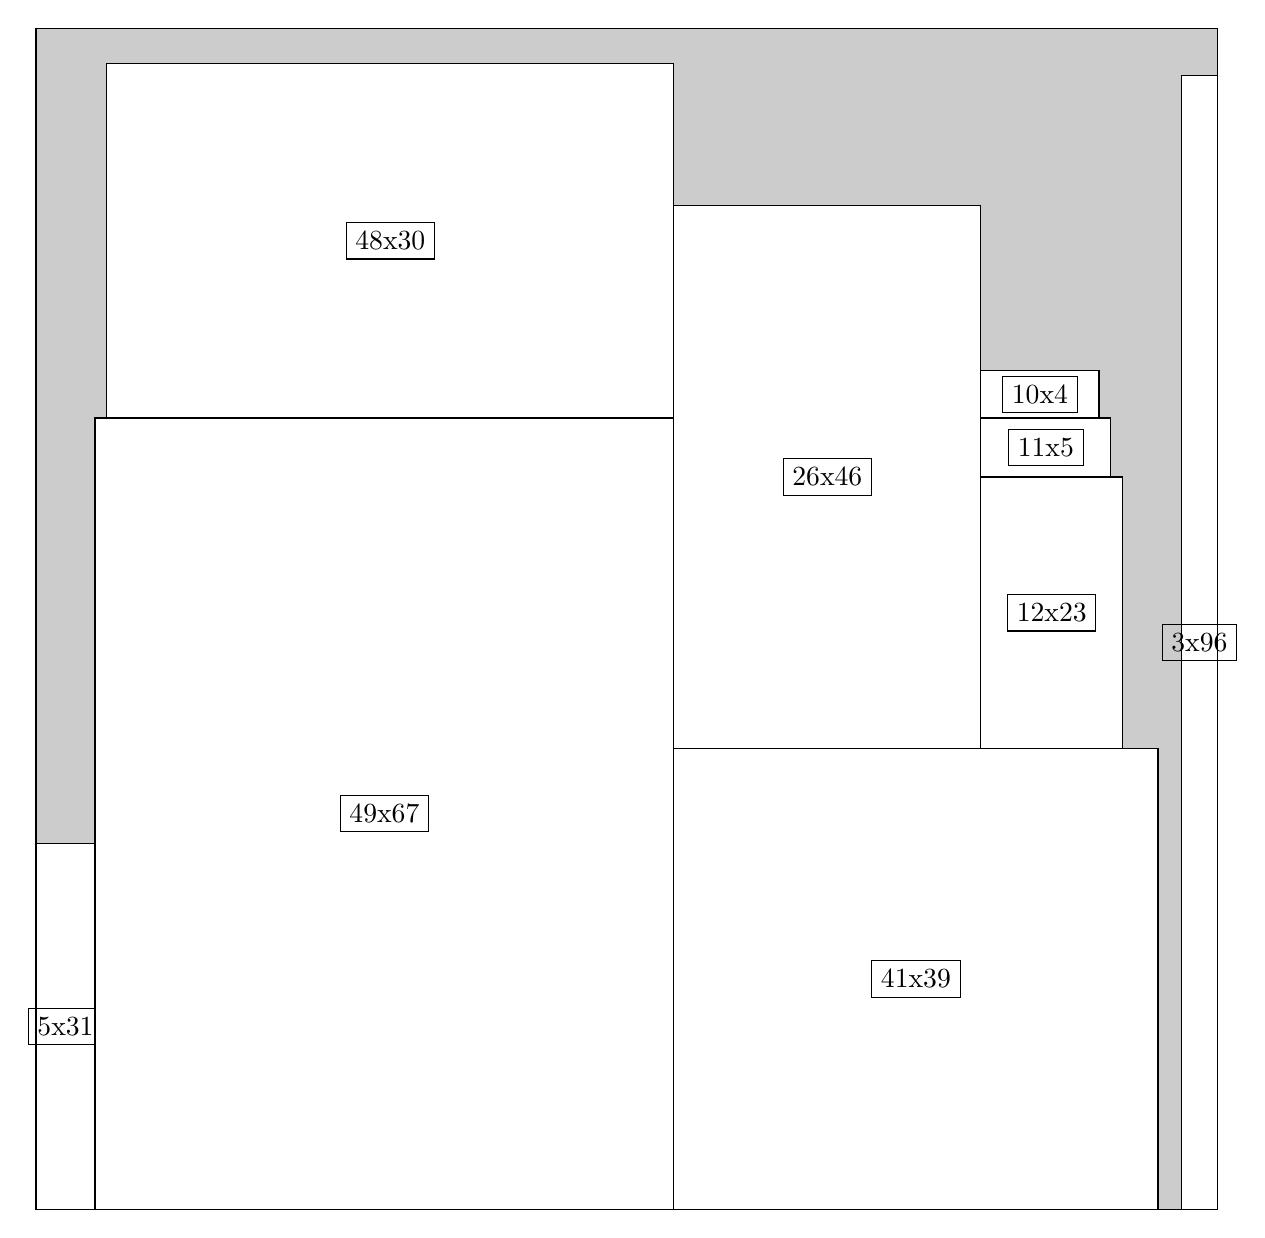
\begin{tikzpicture}[shorten >=1pt,scale=1.0,every node/.style={scale=1.0},->]
\tikzstyle{vertex}=[circle,fill=black!25,minimum size=14pt,inner sep=0pt]
\filldraw[fill=gray!40!white, draw=black] (0,0) rectangle (15.0,15.0);
\foreach \name/\x/\y/\w/\h in {5x31/0.0/0.0/0.75/4.6499999999999995,49x67/0.75/0.0/7.35/10.049999999999999,41x39/8.1/0.0/6.1499999999999995/5.85,48x30/0.8999999999999999/10.049999999999999/7.199999999999999/4.5,26x46/8.1/5.85/3.9/6.8999999999999995,3x96/14.549999999999999/0.0/0.44999999999999996/14.399999999999999,12x23/12.0/5.85/1.7999999999999998/3.4499999999999997,11x5/12.0/9.299999999999999/1.65/0.75,10x4/12.0/10.049999999999999/1.5/0.6}
\filldraw[fill=white!40!white, draw=black] (\x,\y) rectangle node[draw] (\name) {\name} ++(\w,\h);
\end{tikzpicture}


w =5 , h =31 , x =0 , y =0 , v =155
\par
w =49 , h =67 , x =5 , y =0 , v =3283
\par
w =41 , h =39 , x =54 , y =0 , v =1599
\par
w =48 , h =30 , x =6 , y =67 , v =1440
\par
w =26 , h =46 , x =54 , y =39 , v =1196
\par
w =3 , h =96 , x =97 , y =0 , v =288
\par
w =12 , h =23 , x =80 , y =39 , v =276
\par
w =11 , h =5 , x =80 , y =62 , v =55
\par
w =10 , h =4 , x =80 , y =67 , v =40
\par
\newpage


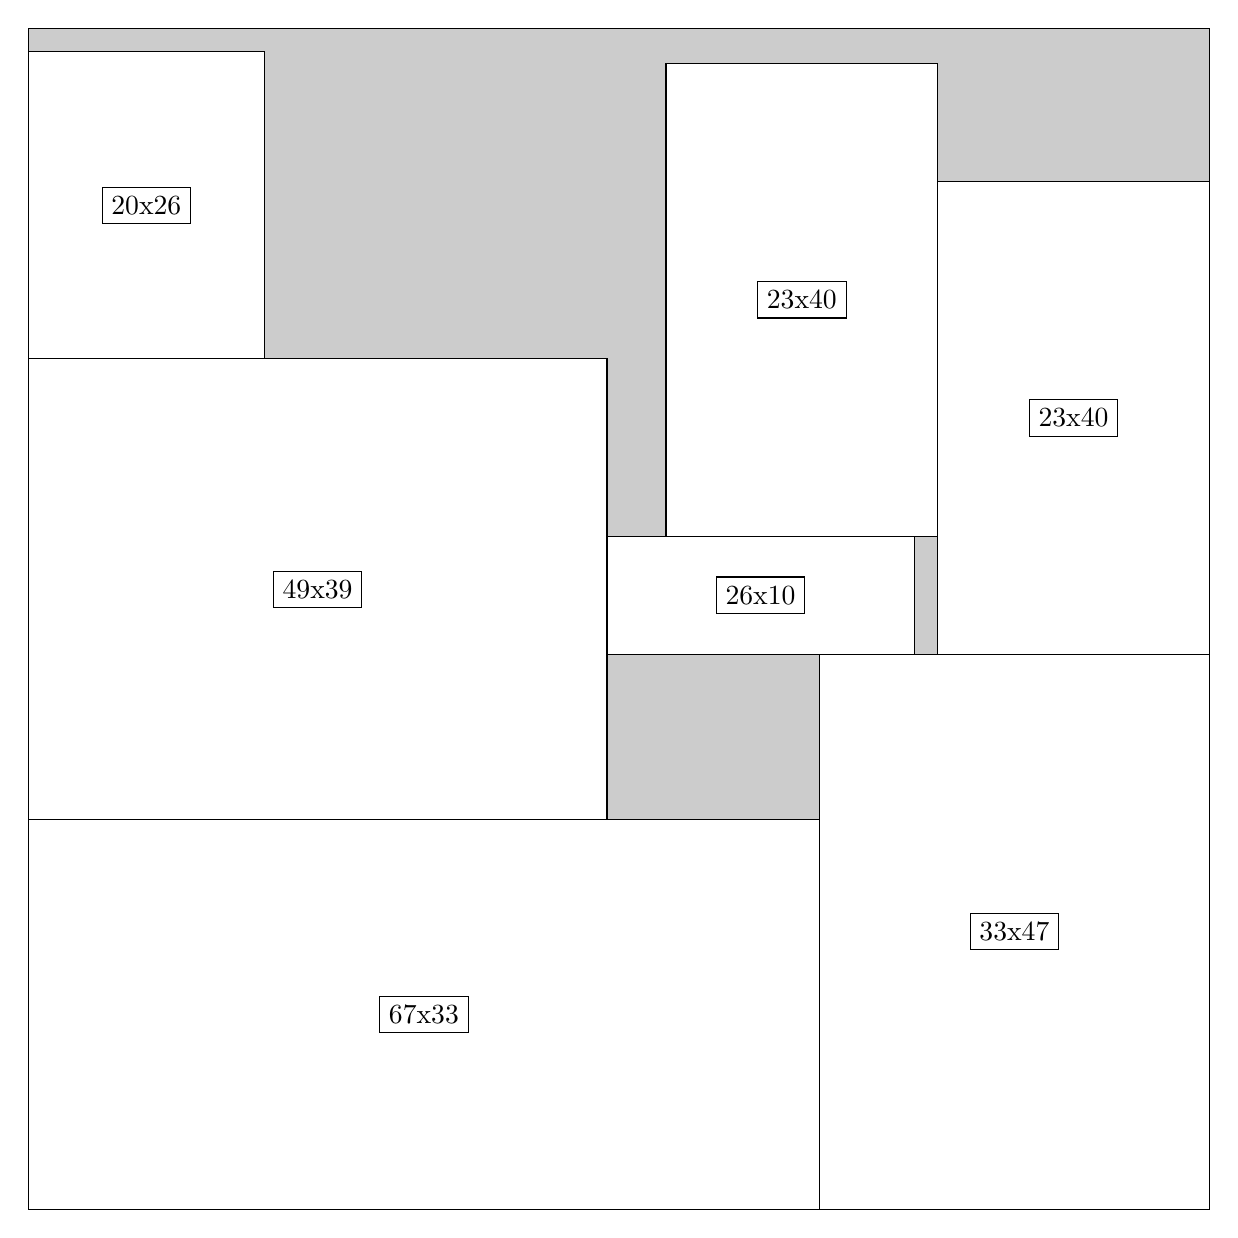
\begin{tikzpicture}[shorten >=1pt,scale=1.0,every node/.style={scale=1.0},->]
\tikzstyle{vertex}=[circle,fill=black!25,minimum size=14pt,inner sep=0pt]
\filldraw[fill=gray!40!white, draw=black] (0,0) rectangle (15.0,15.0);
\foreach \name/\x/\y/\w/\h in {67x33/0.0/0.0/10.049999999999999/4.95,49x39/0.0/4.95/7.35/5.85,33x47/10.049999999999999/0.0/4.95/7.05,23x40/11.549999999999999/7.05/3.4499999999999997/6.0,23x40/8.1/8.549999999999999/3.4499999999999997/6.0,20x26/0.0/10.799999999999999/3.0/3.9,26x10/7.35/7.05/3.9/1.5}
\filldraw[fill=white!40!white, draw=black] (\x,\y) rectangle node[draw] (\name) {\name} ++(\w,\h);
\end{tikzpicture}


w =67 , h =33 , x =0 , y =0 , v =2211
\par
w =49 , h =39 , x =0 , y =33 , v =1911
\par
w =33 , h =47 , x =67 , y =0 , v =1551
\par
w =23 , h =40 , x =77 , y =47 , v =920
\par
w =23 , h =40 , x =54 , y =57 , v =920
\par
w =20 , h =26 , x =0 , y =72 , v =520
\par
w =26 , h =10 , x =49 , y =47 , v =260
\par
\newpage


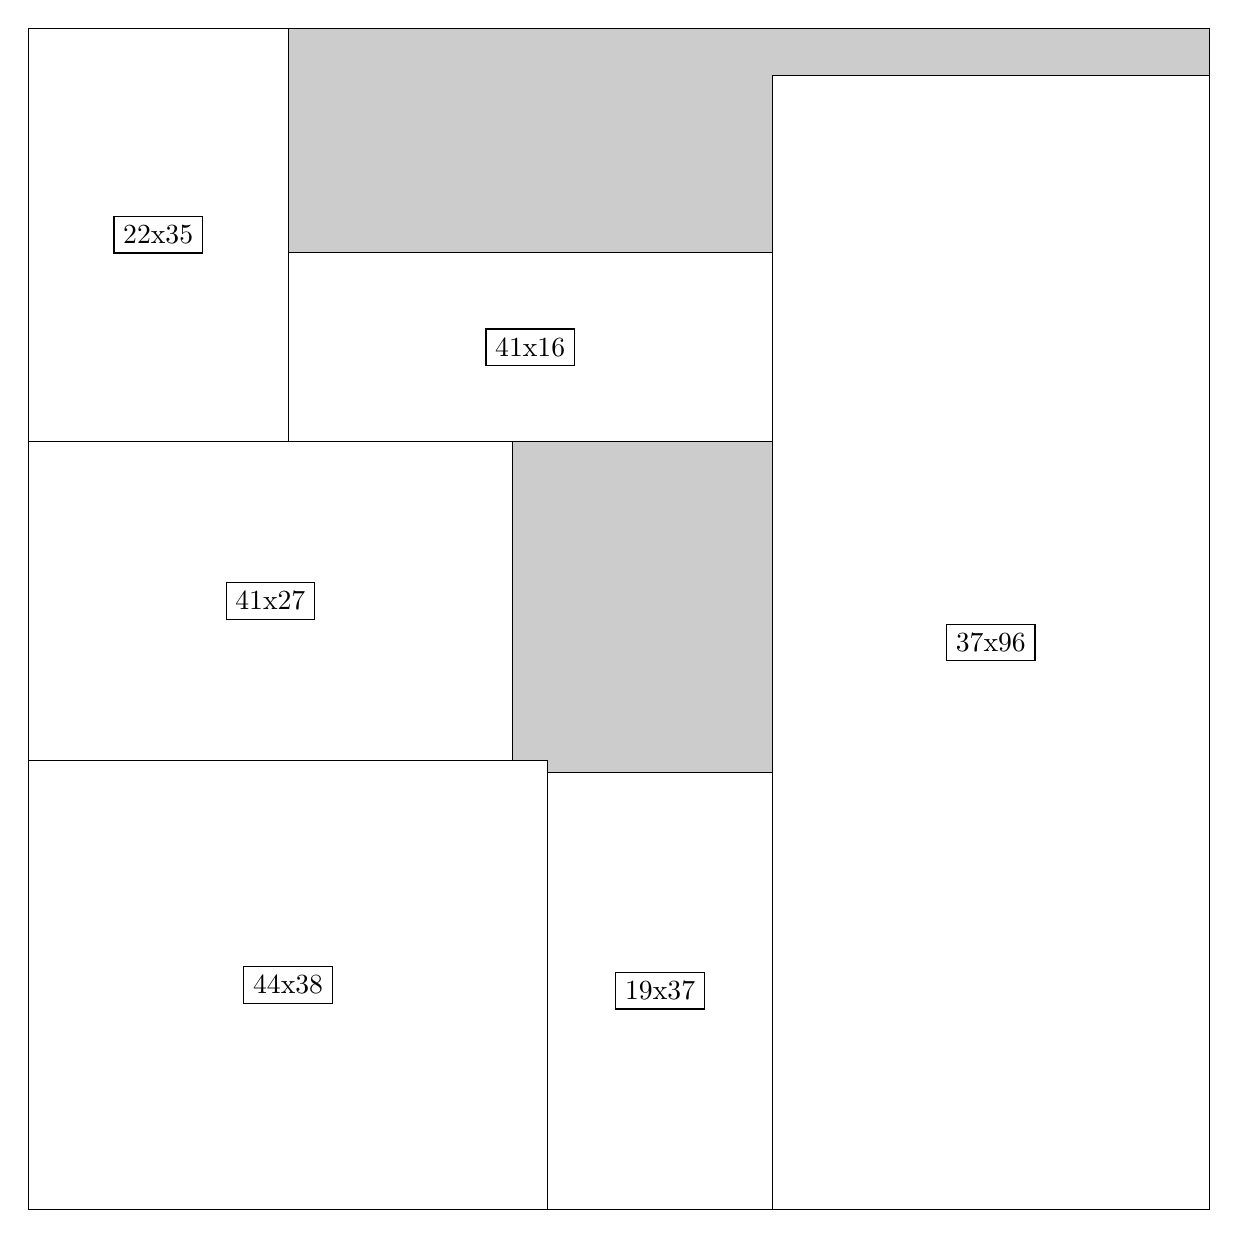
\begin{tikzpicture}[shorten >=1pt,scale=1.0,every node/.style={scale=1.0},->]
\tikzstyle{vertex}=[circle,fill=black!25,minimum size=14pt,inner sep=0pt]
\filldraw[fill=gray!40!white, draw=black] (0,0) rectangle (15.0,15.0);
\foreach \name/\x/\y/\w/\h in {44x38/0.0/0.0/6.6/5.7,41x27/0.0/5.7/6.1499999999999995/4.05,22x35/0.0/9.75/3.3/5.25,19x37/6.6/0.0/2.85/5.55,41x16/3.3/9.75/6.1499999999999995/2.4,37x96/9.45/0.0/5.55/14.399999999999999}
\filldraw[fill=white!40!white, draw=black] (\x,\y) rectangle node[draw] (\name) {\name} ++(\w,\h);
\end{tikzpicture}


w =44 , h =38 , x =0 , y =0 , v =1672
\par
w =41 , h =27 , x =0 , y =38 , v =1107
\par
w =22 , h =35 , x =0 , y =65 , v =770
\par
w =19 , h =37 , x =44 , y =0 , v =703
\par
w =41 , h =16 , x =22 , y =65 , v =656
\par
w =37 , h =96 , x =63 , y =0 , v =3552
\par
\newpage


\end{document}